\documentclass[10pt]{article}
\usepackage{ctex}
\usepackage{graphicx}
\graphicspath{{E:/大学课程/大一下/人工智能程序设计/作业集/第一次作业/},{pics/}}
\usepackage{amsmath}
\usepackage{amssymb}
\usepackage{float}%使图片紧跟在文字后面


\title{第一周平时作业}
\author{朱士杭\ 231300027}
\date{\kaishu \today}

\begin{document}
	\maketitle
\section{问题一}
	\subsection{强类型语言与弱类型语言}
		\subsubsection{强类型语言}
	对于一种语言而言如果里面的变量被定义为某一种数据类型之后,除非人为对其进行强制类型转换,否则其数据类型不会发生改变,那么该语言就称为强类型语言
		\subsubsection{弱类型语言}
	如果这种语言里面的变量被定义之后,在不同的场景之下可以灵活类型转换,不会在一开始特别定义其数据类型
	\subsection{动态类型语言与静态类型语言}
		\subsubsection{动态类型语言}
	程序在运行期间才会检查数据类型,在写脚本的时候不需要对变量进行类型声明,比如说python是解释器不需要编译那么在遇到一个变量定义的时候比如说a=3.0自动将a的数据类型定义为float
		\subsubsection{静态类型语言}
	程序在编译期间就会检查所有的数据类型,在写脚本的时候需要对每个变量进行显示的类型声明,比如说C++中double a=3.0需要对a的数据类型进行说明以便于编译器之后进行类型的检查
	
	ps补充说明:问题一开始并不知道答案,参考过相关资料,链接如下:https://zhuanlan.zhihu.com/p/62570358 但是答案都是自己看完以后自己总结之后写上去的   养成学术诚信的好习惯
	
\section{问题二}
	\subsection{编译执行和解释执行}
		\subsubsection{编译执行}
	编译器会先将脚本转换为编译语言,然后生成经过绑定联结之后生成一个exe的可执行文件,此时就会脱离原来的脚本,即使电脑没有配置相应的语言也可以执行 \par
	优点是编译执行效率高,占用资源小,适合复杂程序的开发\par
	缺点严重依赖环境与操作系统,比如在Windows上的编译程序直接迁移到Linux系统上会执行不了
		\subsubsection{解释执行}
	不需要编译器,程序会根据脚本一行一行执行下去,不会生成相应的可执行文件,如果出现bug会立即终止程序,需要有相应的语言环境比如python \par
	优点是执行的时候不依赖于环境\par
	缺点是一句一句执行会造成计算机资源的浪费,执行效率低
	
\section{问题三}
	\begin{figure}[htbp]
		\centering
		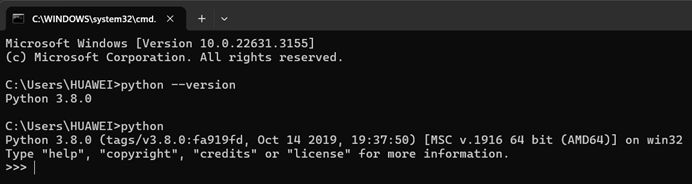
\includegraphics[scale=1]{python3.8版本查看}
		\caption{python3.8版本查看}
	\end{figure}
	\begin{figure}[htbp]
		\centering
		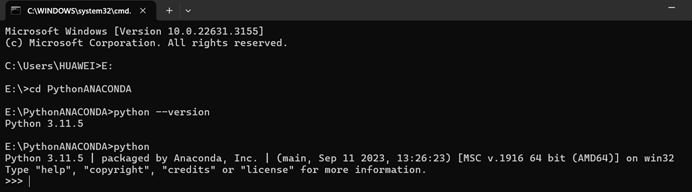
\includegraphics[scale=1]{python3.11版本查看}
		\caption{python3.11版本查看}
	\end{figure}
	ps补充说明:自己在电脑里面安装了四个版本的python,分别是3.8、3.9、3.11、3.12但是不知道为什么cmd里面只显示3.8的版本(估计是默认版本吧),之后又切换到了3.11的文件夹下,显示出3.11版本(用的是pycharm和anaconda配置的环境)
	
\section{问题四——不同方式使用Python}
	\begin{figure}[H]
		\centering
		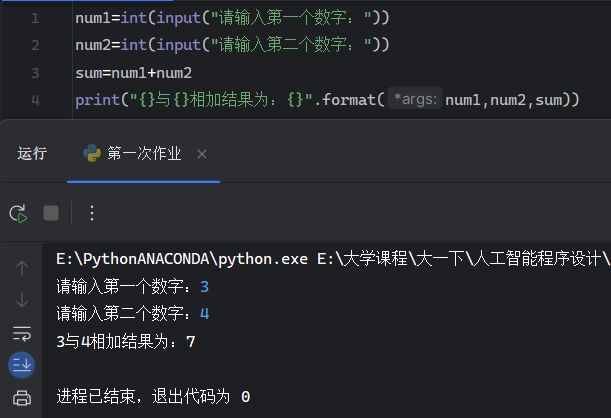
\includegraphics[scale=0.6]{用文件方式编写的相加}
		\caption{用文件方式编写的相加}
	\end{figure}
	\begin{figure}[H]
		\centering
		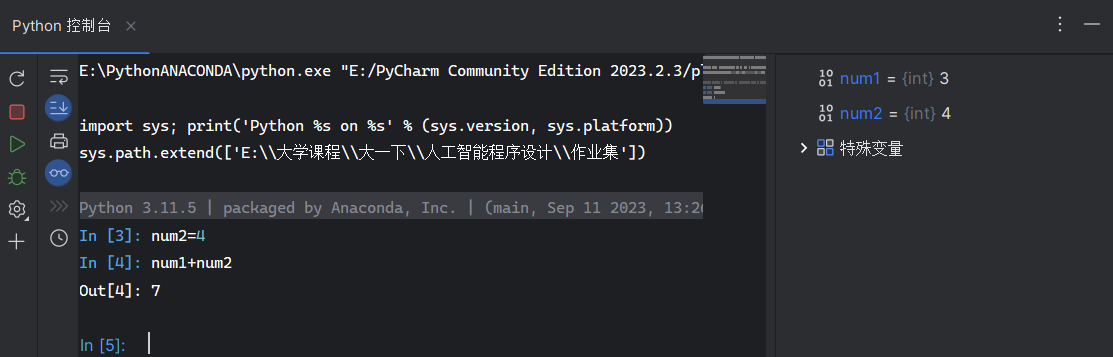
\includegraphics[scale=0.55]{用交互模式编写相加}
		\caption{用交互模式编写相加}
	\end{figure}


	
\section{问题五——使用help命令}
	\begin{figure}[H]
		\centering
		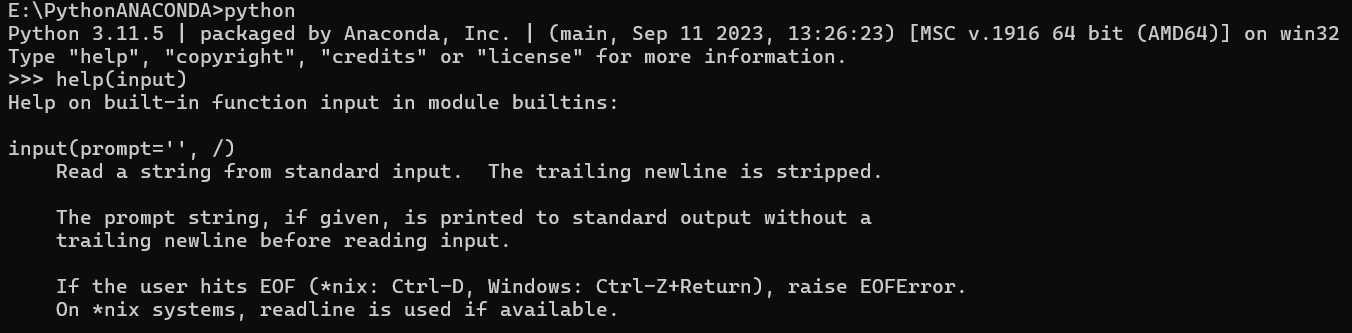
\includegraphics[scale=0.45]{help_input}
		\caption{help(input)}
	\end{figure}
	\begin{figure}[H]
		\centering
		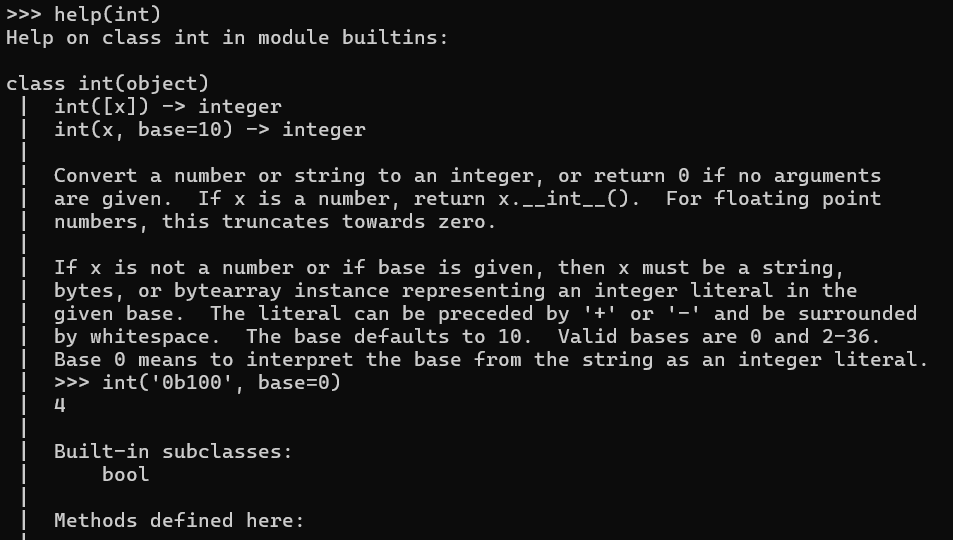
\includegraphics[scale=0.45]{help_int}
		\caption{help(int)}
	\end{figure}
	\begin{figure}[H]
		\centering
		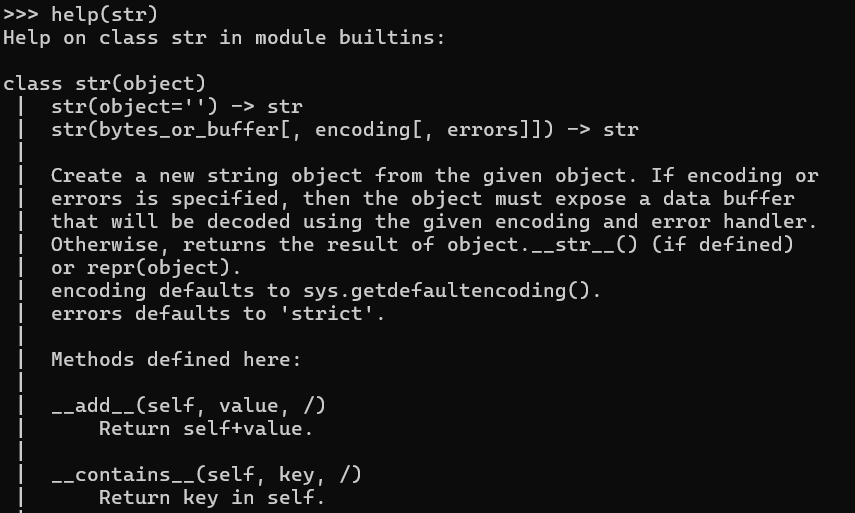
\includegraphics[scale=0.45]{help_str}
		\caption{help(str)}
	\end{figure}




\section{后记}
	这是我第一次使用LaTeX写作业,不足之处敬请谅解,之后会不断提升使用LaTeX的技术,在此纪念一下第一次使用这样的工具,就像我们第一次用Python和C++打印出“HelloWorld”一样弥足珍贵
	
	
\end{document}